\chapter{Background and Motivation}
\label{chap:backgrd}
%explain structure of this thesis
Nowadays neural networks and deep learning has become a hot topic in pattern recognition, speaker identification, image processing and many other fields. In this thesis, deep neural networks are used as a solution for sound type classification problem.
In Chapter \ref{chap:backgrd} some basic concepts related to sound type classification and neural networks are introduced. This thesis is based on part of works of the Two!Ears system. Sound type classification is a module of the Two!Ears system. These basic concepts are introduced in section \ref{sec:soundtc}. Section \ref{sec:deepNN} explains what DNNs are and introduces the Caffe framework, which is used for producing the experiment results in this thesis. After that, the main part of the thesis starts by exploring the architecture of neural networks applied to sound type classification. Three types of architectures are discussed in Chapter \ref{chap:architecture}. A good architecture doesn't solve the problem completely, overfitting is always a problem one should consider in machine learning problems. In Chapter \ref{chap:dataAug}, data augmentation is introduced to deal with the overfitting problem. Tuning parameters of deep neural networks requires a broad and lengthy exploration of the parameter space.  At last, a conclusion is drawn in Chapter \ref{chap:conclusion}. I will also talk about future works related to this topic.

\section{Sound Type Classification}
\label{sec:soundtc}
%goal:usually features are handcrafted by domain experts
In this thesis, sound type classification is a supervised machine learning problem, which serves as a module of the Two!Ears System. The training data set is the NIGENS(NI General Sound) Database. In this section I will explain the sound type classification based on the six steps of supervised learning problem\cite{mohri2012foundations}
\begin{itemize}
	\item Determine the type of training examples.
	\item Gather a training set.
	\item Determine the input feature representation of the learned function.
	\item Determine the structure of the learned function and corresponding learning algorithm.
	\item Run the learning algorithm on the gathered training set.
	\item Evaluate the accuracy of the learned function on the test set.
\end{itemize}

\subsection{NIGENS Database} 
NIGENS is short for 'NI General Sound'.\cite{twoearsprojectdoc} NIGENS was compiled from the Stockmusic\footnote{Stockmusic is the online redistributor of the famous Sound Idea’s sounds library, offering individual files rather than precompiled collections. See http://www.stockmusic.com/sound\_effects}
sounds archive. The database consists of 11 classes of everyday sounds(alarm, crying baby, crash, barking dog, running engine, female speech, burning
fire, footsteps, knocking on door, ringing phone, piano) and a class of general 'anything else'. For each of these 11 classes of everyday sounds, 50 wav files were selected. For the general sound class, 237 wav files were selected. Briefly, the NIGENS database is constructed from 787 high quality sound files.


In this thesis, the NIGENS Database is used as the training dataset for sound type classification. 
\subsection{The Two!Ears System}
%idea\
%representations(amsFeatures,ratemaps)\\
%{Feature extraction}\\
%{Classification}\\
%LASSO methods\\
The Two!Ears system works on auditory modeling by a systemic approach.\footnote{The official website of the Two!Ears System: http://twoears.eu/} The goal of this project is to develop an intelligent, active computational model of auditory perception and experience in a multi-modal context. 
In order to construct such a system for dynamic interaction application, a dynamic auditory scene analysis model is needed. In this model, sound type classification extracts one of the important attributes, the sound type, of corresponding aural objects.

In speak of determining the input feature representation for the sound type classification module of the Two!Ears System, rate maps, spectral features, amplitude modulation spectrogram features and onset strengths have all been used as input feature representation in previous work. These features are extracted using the auditory front-end in the Two!Ears system. However the full combination of all these features may contain redundant information and it requires a long training duration. In this thesis, the combination of rate maps and AMS(Amplitude Modulation Spectrogram) features are determined as the input feature representation to shorten the training time.

\subsubsection*{Rate maps}
Rate maps are biologically inspired spectrogram-like maps over time and frequency domain, which are supposed to represent auditory nerve firing rate. Rate maps are computed by smoothing the corresponding inner hair cell signal representation with a leaky integrator. The rate maps features used in this thesis are extracted from 16 frequency channels for each of the 63 time frames. 

The rate maps extracted from NIGENS together with the target labels are stored in HDF5 files. The rate maps for all the training segments are stored as a multidimensional array with size  $N\times 1\times 63\times 16$. $N$ is the number of training sound sources. $63$ indicates the length of sound sources in time frames and $63$ time frames is a one second sound block.  $16$ is the number of frequency channels.

\subsubsection*{AMS features}
AMS is the abbreviation for 'Amplitude Modulation Spectrogram'.  The human auditory system is able to focus
on a desired target source and to segregate it from interfering background noise.
Currently the ideal segregation of noisy speech, as represented by the IBM(Ideal binary mask), was estimated by only exploiting AMS features\cite{may2014computational}. Instead of linearly-scaled modulation filters, an auditory-inspired modulation filterbank with logarithmically-scaled modulation filters are used here.
 Each frequency channel of the auditory spectrogram was processed by a second-order low-pass filter with a cutoff frequency of 4 Hz and 8 second-order band-pass filters with center frequencies spaced logarithmically between 8 and 1024 Hz, altogether representing a
modulation filterbank, which produces the final set of 9 logarithmically-scaled AMS features for each frequency channel\cite{twoearsprojectdoc}.

The AMS features extracted from NIGENS together with the target labels are stored in HDF5 files. The AMS features are stored as a multidimensional array with size  $N\times 9\times 63\times 16$. Similar to the rate maps array, $N$ is the number of training sound sources. $9$ is the number of modulation filters. $63$ represents the length of sound sources in time frames. $16$ indicates the number of frequency channels.

\subsubsection*{LASSO Binary Classifier}
With previously mentioned features, it is quite easy to construct a binary classifier. In previous stage of the project, some approaches are developed to achieve this sound type classification task. One of the identification pipeline looks like this:

\begin{figure}[h!]
	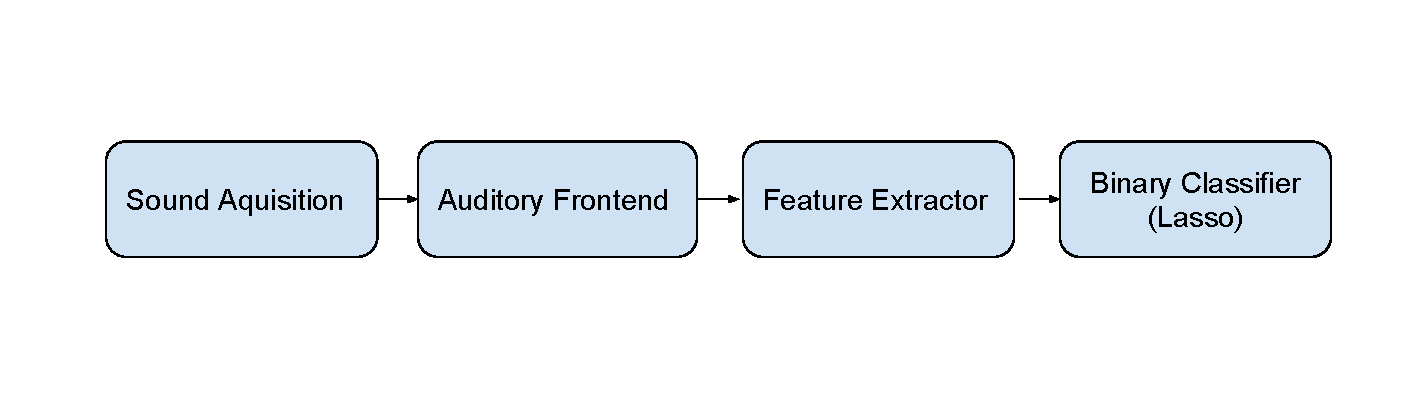
\includegraphics[scale=0.5]{../image/chapter1/identification-pipeline.pdf}
	\caption{Identification Pipeline}
	\label{fig:id-pipeline}
\end{figure}

%TODO: LASSO NOMENCLATURE
In this pipeline, 11 binary one-against-all classifiers using LASSO regression method are trained to accomplish this task. For each of these 11 classes of sound types, a corresponding classifier takes the previously mentioned features $\underline{\mathbf{x}}$ as input and outputs a binary value $y\in \lbrace0,1\rbrace$, where $1$ represents target label. With all of the 11 binary outputs, we can construct a binary vector. An all-zero vector means the sound source is classified as 'anything else' class. This method enables multi-label classification, which means a sound source may be classified as a mix of several classes. 

The accuracy performance of LASSO binary classifier is displayed in Tab.\ref{fig:lassclf}.\footnote{This tabular is extracted from the group talk presentation by Dr. Johannes Mohr on 22.April.2016}%TODO source
Here we use sensitivity, specificity and balanced accuracy to evaluate the classification performance. These three performance metrics are calculated according to the formular below:
\begin{align*}
	sensitivity &= \frac{\#TruePositive}{\#Positive}\\
	specificity &= \frac{\#TrueNegative}{\#Negative}\\
	balanced\quad accuracy &= \frac{sensitivity+specificity}{2}
\end{align*}
As we can see from the bar chart,  Fig.\ref{fig:lassclf}, LASSO classifier performs quite well for class 'female speech', where it achieves $100\%$ sensitivity and $100\%$ specificity. However, the performance of this binary classifier is not so satisfying at class 'engine' with $66\%$ sensitivity and $82\%$ specificity. 

\begin{figure}[h!]
\caption{LASSO Binary Classification Performance}
\label{fig:lassclf}
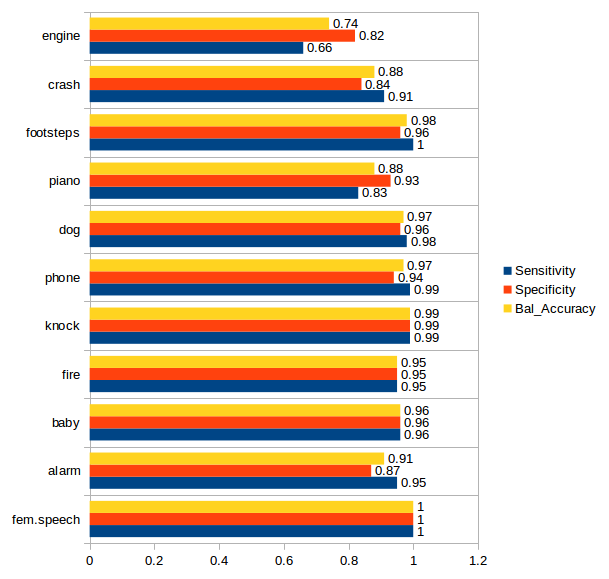
\includegraphics{../image/chapter1/LASSO_results.png}
\end{figure}

\section{Deep Neural Networks}
\label{sec:deepNN}
%motivation(DNN can learn features rather than define them->compare to sec.1.2.2)\\
%related applications,\\
%subsections for DNN(components introduction,caffe)
\subsection{Motivation}
In previous sections, we've seen LASSO binary classifier as a solution to sound type classification problem. In the sound type classification module of the Two!Ears system, handcrafted features(rate maps and AMS features) are taken as the input feature vectors of LASSO binary classifiers. In such simply structured supervised learning model, the quality of features is critical. However, the choice of good features is quite difficult. 

Instead of keeping working hard on feature selection, we now introduce deep neural networks(DNNs) to solve the problem. DNNs can learn features with multiple layers and find high level abstractions in data rather than simply using handcrafted features. Because of such excellent characteristic, DNNs are widely used in a variety of machine learning applications. For example, in automatic speech recognition, DNNs are used to train bottleneck features\cite{zhang2014extracting}. Also in computer vision, DNNs are excellent at learning a good representation of the visual inputs, which can be used to do semantic image segmentation\cite{krizhevsky2012imagenet}. 
\subsection{DNN Structures}
%TODO
A deep neural network (DNN) is an artificial neural network (ANN) with multiple hidden layers of units between the input and output layers\cite{bengio2009learning}\cite{schmidhuber2015deep}. Each layer is made of neurons with learnable weights and biases as parameters of the whole network. Each neuron takes the inner product of outputs from previous layers or input feature vectors with corresponding weights as input and applies an activation function. The common choice of the activation function is the sigmoid function. Fig.\ref{fig:dnnstruc} shows a regular deep neural network structure. If all of the neurons in each layer of the network are fully connected to all activation neurons in the previous layer, such a network is called fully connected neural network.
\begin{figure}
	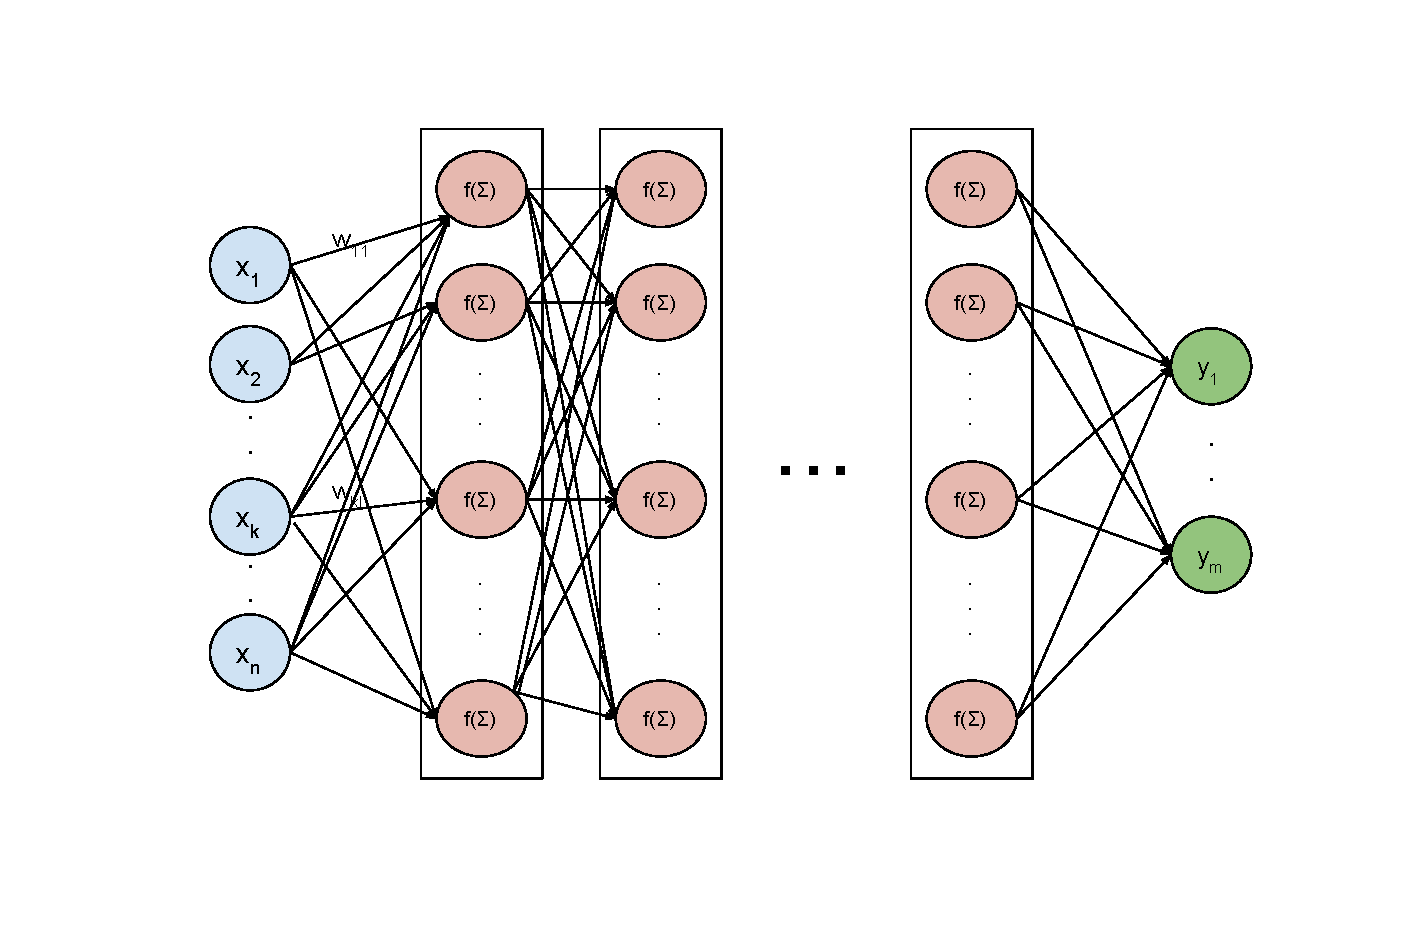
\includegraphics[scale=0.5]{../image/chapter1/dnnstruc.pdf}
	\caption{Deep neural network structure}
	\label{fig:dnnstruc}
\end{figure}

However, such structure is not so efficient with multi-dimensional data like images. Considering a fully connected neural network, the amount of paramters increases with the size of inputs and the number of hidden layers. Too many parameters during training process usually leads to overfitting problem. In this thesis, a variant of regular DNN ,convolutional neural network(CNN), is constructed to solve the problem.

\subsubsection*{Convolutional Neural Networks}
\textit{Convolutional Neural Networks (CNN) are biologically-inspired variants of MLPs(Multilayer Perceptron). }\cite{deeplrn01}

The layers of a CNN have neurons arranged in 3 dimensions: width, height, depth. Instead of following the full connection manner, the neurons of layers in CNNs will be only connected to a small region of layer before it. Such region is called receptive field. In this way, the amount of parameters to be learned is decreased compared with fully connected neural networks. Also parameter sharing scheme is used in Convolutional Layers to control the number of parameters\cite{lecun1995convolutional}. In each layer a new data volume is constructed with corresponding layer parameters. At last, an output volume, which is usually one dimensional vector, is constructed as the final output score.

\subsection{Caffe Toolbox}
Caffe\cite{jia2014caffe} is a deep learning framework. It is developed by the Berkeley Vision and Learning Center (BVLC) and by community contributors. Yangqing Jia created the project during his PhD at UC Berkeley. Caffe is released under the BSD 2-Clause license. In this thesis, I used caffe as the toolbox to implement the convolutional neural networks for sound type classification.

Caffe is written in C++ and it also provides the users with command line, Python, and MATLAB interfaces. The command line interface is the caffe tool for model training, scoring, and diagnostics. All training requires a solver configuration file. In this configuration file, the optimization method and its corresponding parameters are defined. To create a Caffe model you need to define the model architecture in a protocol buffer definition file. In solver configuration file, the full path of the model architecture definition file should also be defined.\footnote{For further details, please refer to the official website of caffe:http://caffe.berkeleyvision.org/}

Caffe provides a variety of layers for users. Generally there are 5 types of layers: vision layers, loss layers, activation/neuron layers, data layers and common layers.
\begin{itemize}
\item  Vision Layers:\\
Convolution, Pooling, Local Response Normalization(LRN),im2col\\
Vision layers  take images as input and produce new images as output. In this thesis, Convolution and Pooling layers were used.
\item Loss Layers:\\
\\Softmax, Sum-of-Squares/Euclidean, Hinge/Margin, Sigmoid Cross-Entropy, Infogain, Accuracy and Top-k\\
Loss layers compare an output to a target and assign cost. During the training stage, the loss itself is computed by the forward pass and the gradient w.r.t. the loss is computed by the backward pass. In this way, loss layer drives the learning process by minimizing the loss. In this thesis, Softmax and Sigmoid Cross-Entropy were used.

\item Activation/Neuron Layers:\\ 
ReLU / Rectified-Linear and Leaky-ReLU, Sigmoid,TanH / Hyperbolic Tangent,Absolute ,Power,BNLL\\
Activation / Neuron layers are element-wise operators, taking one bottom blob and producing one top blob of the same size. In this thesis, ReLU and Sigmoid layers were used.
\item Data Layers:\\
Database, In-Memory, HDF5 Input, HDF5 Output, Images, Windows, Dummy\\
Data enters Caffe through data layers.  Use different types of data layers w.r.t different data sources. In this thesis,HDF5Data layers was used, as the handcrafted features, rate maps and AMS features, were written into hdf5 files.
\item Common Layers:\\
InnerProduct,Splitting,Flattening,Reshape,Concatenation,Slicing, Elementwise Operations,Argmax,Softmax,Mean-Variance Normalization
\\
Common Layers are implemented for simple data operations.
In this thesis, InnerProduct, Concatenation,Slicing and Sigmoid layers were used.
\end{itemize}


\section{Aims of Thesis}
In my thesis, I investigate different architectures of DNNs and different loss functions to improve the  performance of this sound type classification system. I also tried to use data augmentation to overcome the overfitting problem.
